\documentclass{article}
\usepackage[T1]{fontenc}

\usepackage{graphicx}
\usepackage{listings}
\begin{document}

\title{FOSS Lab Report - GIT Version Control System}
\author{Gokul K\\[2\baselineskip]
Roll Number: 21\\[2\baselineskip]}
\date{5 April 2020}

\maketitle

\newpage

\tableofcontents

\newpage

\setcounter{section}{27}
\subsection{Aim}
To try Version Control System setup and usage using GIT\newline
1. Creating a repository\newline
2. Checking out a repository\newline
3. Adding content to the repository\newline
4. Committing the data to a repository\newline
5. Updating the local copy\newline
6. Comparing different revisions\newline
7. Revert\newline
8. Conflicts and a conflict Resolution\newline
\newpage

\subsection{Installation}
To install git in Arch-derivative linux distro we need to run:
\begin{verbatim}
	sudo pacman -S git
\end{verbatim}
\newpage

\subsection{Creating a repository}
To start an empty Git repository we need to run the command
\begin{verbatim}
	git init
\end{verbatim}
in the folder we need to initialise the repository
\newline

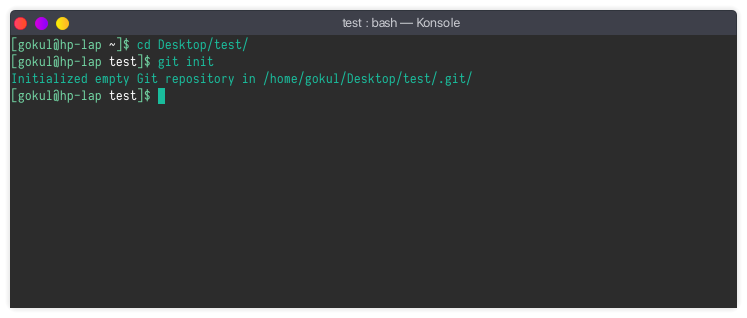
\includegraphics[width=1.2\textwidth]{img/p27/ss1.png}

\newpage
\subsection{Adding content to a repository}
To add a file to a repository, we have to run \begin{verbatim}
	git add filename
\end{verbatim}
Alternatively, we can also provide a folder name in the position of file
name to add a whole directory to the repository.

To add all the files to the repository, we can use
\begin{verbatim}
	git add .
\end{verbatim}

\newpage
\subsection{Commiting the data to a repository}
To commit the files that we have added, we can use\begin{verbatim}
	git commit -m "Commit message"
\end{verbatim}


\subsection{Checking out a repository}
To create a new branch we can use \begin{verbatim}
	git branch branch_name
\end{verbatim}
To checkout out to that branch we have to use \begin{verbatim}
	git checkout branch_name
\end{verbatim}
To create and checkout a branch simultaneously we can also use \begin{verbatim}
 	git checkout -b branch_name
\end{verbatim}
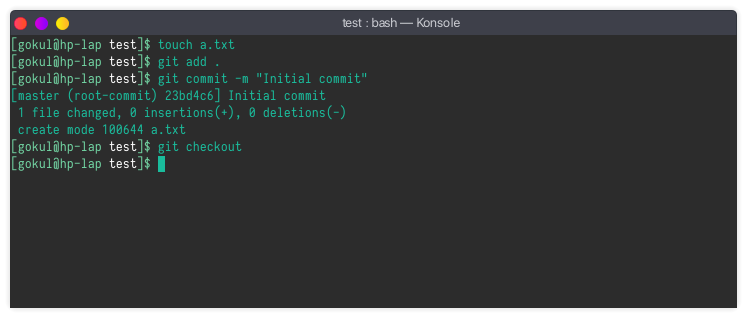
\includegraphics[width=1.2\textwidth]{img/p27/ss2.png}
\newpage

\subsection{Updating the local copy}
If we have specified a remote repository using \begin{verbatim}
	git remote add remotename <url>
\end{verbatim}
we can update the local copy by running \begin{verbatim}
	git pull remotename branchname

\end{verbatim}
\newpage


\subsection{Comparing different revisions}
To compare different commits we can use \begin{verbatim}
	git diff commitid commitid2
\end{verbatim}
where the commitid can be found from \begin{verbatim}
	git log
\end{verbatim}

We can also use \begin{verbatim}
	git diff HEAD filename
\end{verbatim}
To find the changes made from the last commit\newline
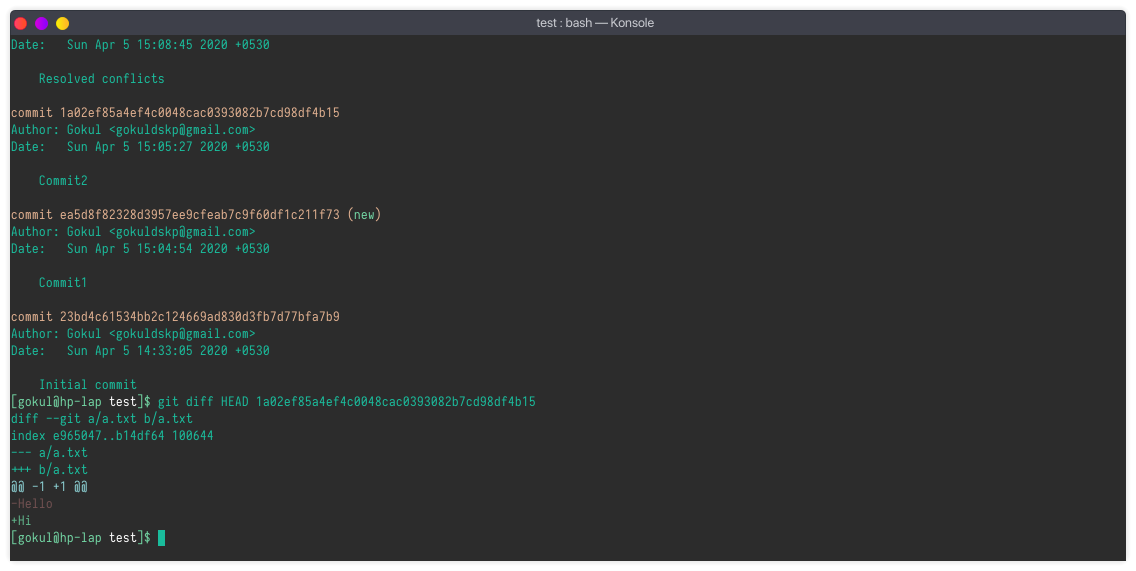
\includegraphics[width=1.2\textwidth]{img/p27/ss7.png}

\newpage
\subsection{Revert}
For reverting to a previous commit, we have to use \begin{verbatim}
	git revert commitref
\end{verbatim}
We have to provide a reference to the commit we need to revert. This will not
delete the commit, but instead it resore the contents of previous commit as a 
new commit.\newline
We have to use reset to delete a commit from the git history

\subsection{Conflicts and a Conflict resolution}
Conflicts arises when we are merging branches containing different versions of
same file.\newline
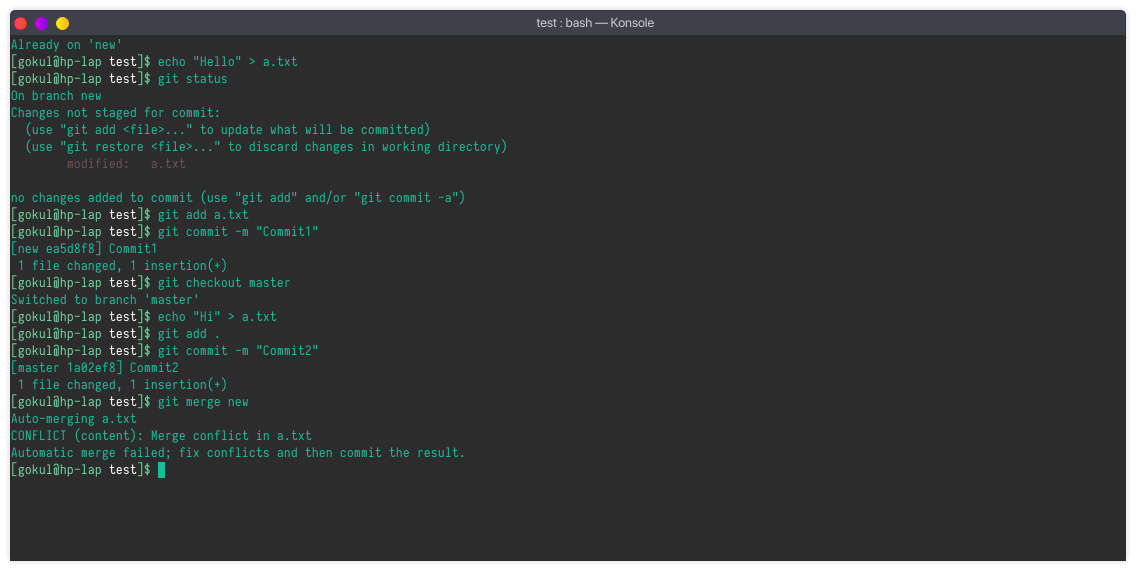
\includegraphics[width=1.2\textwidth]{img/p27/ss3.png}
\newline
We have to resolve the conflict manually using a text editor\newline
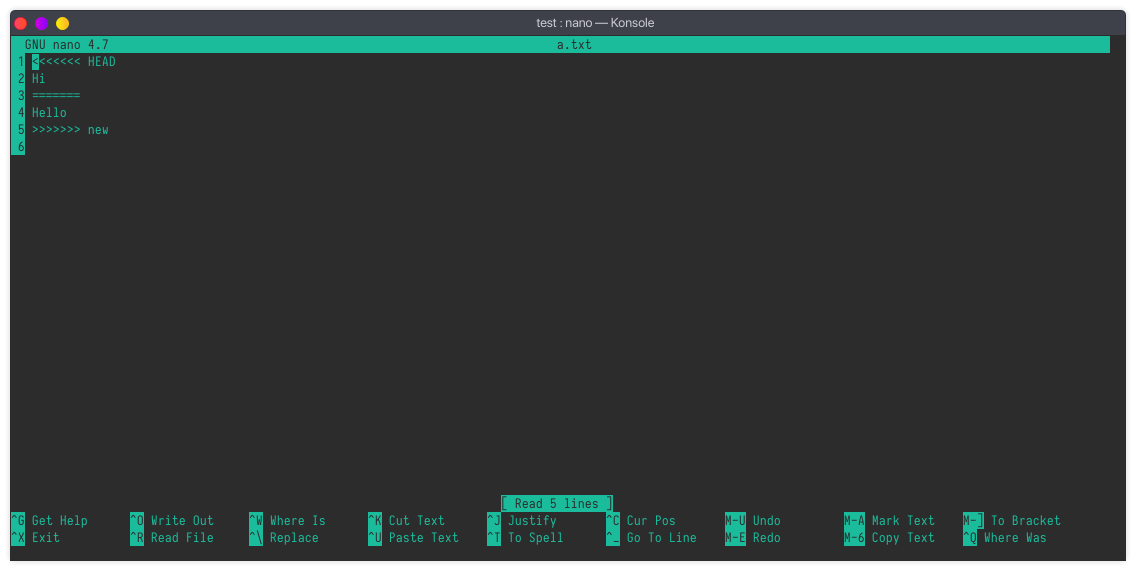
\includegraphics[width=1.2\textwidth]{img/p27/ss4.png}
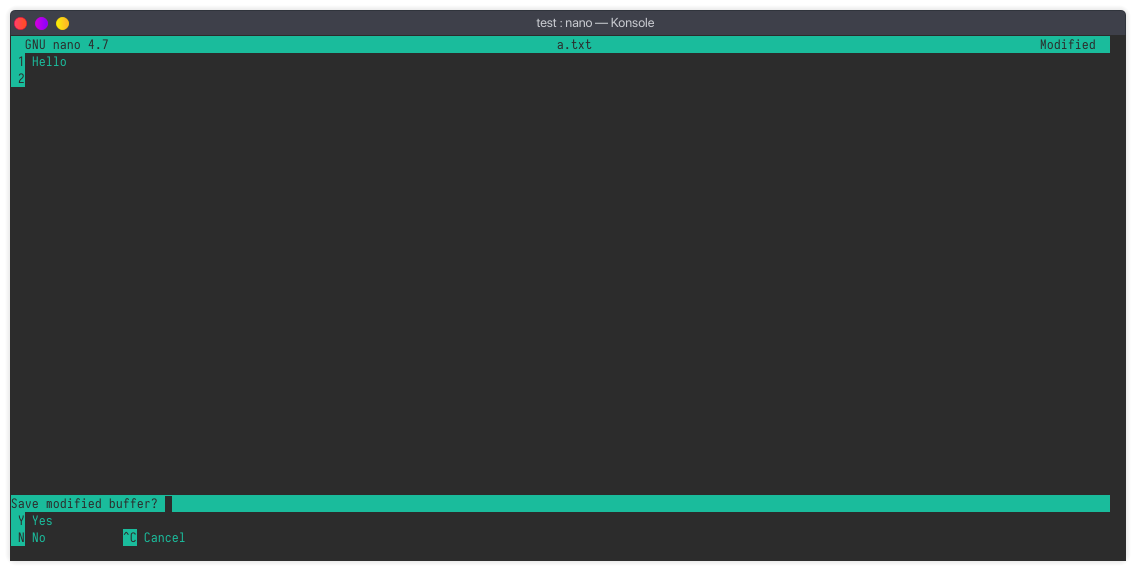
\includegraphics[width=1.2\textwidth]{img/p27/ss5.png}
\newline
Then stage and commit\newline
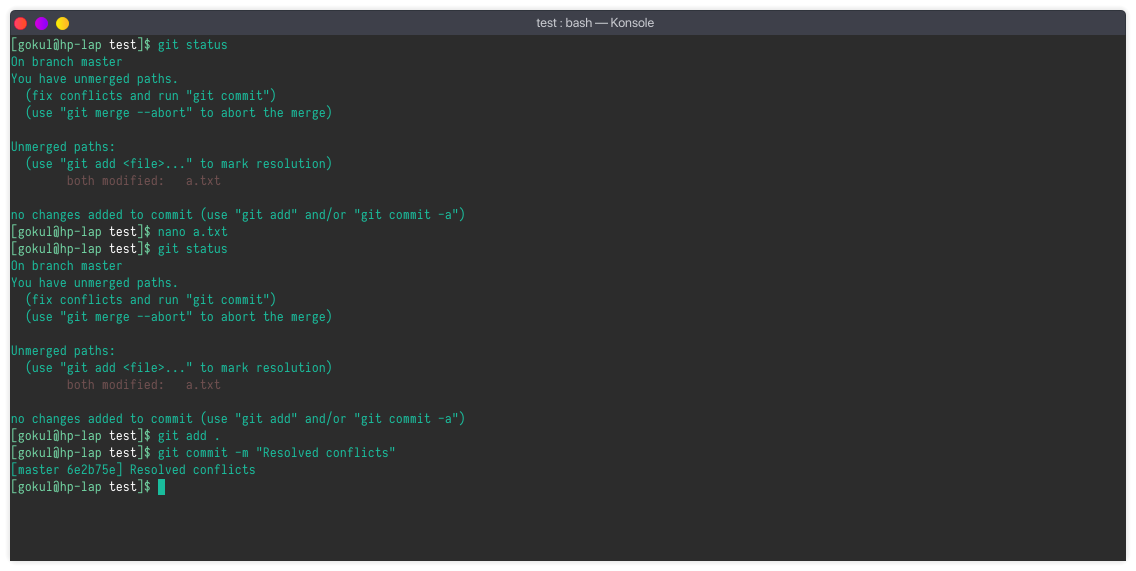
\includegraphics[width=1.2\textwidth]{img/p27/ss6.png}
\newpage
\subsection{Result}
A Git repository is initialised in a folder and different Git commands are tried
on it.
\end{document}